% Exemplo de dissertação usando o modelo do Instituto de Informática da UFRGS
%
% Além de servir como exemplo, este documento tem como finalidade repeoduzir
% o conteúdo e a forma do modelo oficial (em RTF) para uma dissertação de
% mestrado do PPGC.

\documentclass[ppgc,diss]{iiufrgs}

% Pacotes relacionados a codificação de arquivos e de fontes.
\ifxetex
\else
    \usepackage[utf8]{inputenc}
\fi

% Necessário para incluir figuras.
\usepackage{graphicx}

% Pacote para o uso de tabelas.
\usepackage{tabularx}
\usepackage{booktabs}

% Inicialização do hyperref com alguns parâmetros adicionais.
% Use hyperref! Não estamos mais na idade da pedra!
\makeatletter
\hypersetup{%
	hidelinks,
	pdftitle={\@title},
	pdfauthor={\@author},
	pdfcreator={pdfLaTeX},
	bookmarksdepth=4
}
\makeatother

% Referências bibliograficas com o pacote abntex2.
% \usepackage[
%     % Habilita o uso de citações no formato autor-data.
% 	alf,
% 	% O modelo da UFRGS requer que os títulos dos trabalhos estejam em negrito.
%     % Isso é opcional na norma ABNT (que permite que seja usado itálico) e
%     % não é o padrão do abntex2.
%     abnt-emphasize=bf
% ]{abntex2cite}

% Necessario apenas para este exemplo.
\usepackage{framed}

%%%%%%%%%%%%%%%%%%%%%%%%%%%%%%%%%%%%%%%%%%%%%%%%%

% Dados gerais do documento.
\title{
    Normas para apresentação de teses do Instituto de Informática e do PPGC
}

% Esta divisão que coloca "Silva" como sobrenome ao invés de "da Silva" não faz
% muito sentido, mas reflete o modelo da biblioteca.
\author{Silva}{João da}
\advisor[Prof.~Dr.]{Silva}{Orientador da}
\coadvisor[Prof.~Dr.]{Silva}{Co-orientador da}
\date{agosto}{2014}

\keyword{ABNT}
\keyword{Processadores de Texto}
\keyword{Formatação eletrônica de documentos}


\begin{document}

% Cria a folha de rosto.
\maketitle


% Agradecimentos.
\chapter*{Agradecimentos}
Quando desejado pelo autor do trabalho, são apresentados logo após a folha de
rosto, nessa ordem.
São de livre apresentação gráfica.
Geralmente os Agradecimentos são apresentados como um capítulo não numerado.
O mesmo é recomendado para os próximos itens, até o Resumo e Abstract.


% Resumo na língua do documento.
\begin{abstract}
    Consiste na apresentação clara e concisa dos pontos relevantes do trabalho,
    de maneira a permitir ao leitor saber da conveniência ou não da sua leitura na íntegra.
    É redigido pelo autor, em português e em inglês, em páginas distintas.
    Cada resumo ocupará no máximo uma folha e terá até 500 palavras.
    Para maiores informações com relação à redação consultar a NBR 6028 da ABNT.
    Quanto ao estilo, o resumo deve ser composto por uma sequência de frases
    completas e não por uma enumeração de tópicos; a primeira frase deverá ser
    significativa, explicando o tema principal do documento.
    Na redação, dar preferência ao uso da terceira pessoa do singular e do verbo na voz ativa.
    Após o resumo e o abstract devem constar palavras-chave relativas aos assuntos
    da monografia, em português e inglês respectivamente, e separadas entre si por ponto.
\end{abstract}

% Resumo em língua estrangeira.
% Note a ordem dos parâmetros: título traduzido, palavras-chave traduzidas, e
% o corpo do abstract.
% As palavras-chave devem ser separadas por ponto, como manda o modelo.
\begin{englishabstract}
    {This should be in English}
    {ABNT. Text processors. Electronic document preparation.}
    This manual has the purpose of [\ldots].
    Consiste na versão do resumo na língua vernácula para a língua estrangeira.
    As palavras chaves também devem ser traduzidas.
    A versão pode ser em inglês (Abstract), espanhola (Resumen), ou francesa (Résumé).
    O abstract deve apresentar, adicionalmente, uma tradução do título do trabalho.
    O título traduzido é colocado antes do título do capítulo (“Abstract’”), a
    2 cm da margem superior, centralizado, em fonte Times New Roman, tamanho 12 e em negrito.
\end{englishabstract}

% A ordem dos elementos pré-textuais importa.
\listoffigures
\listoftables
\begin{listofabbrv}{UFRGS}
    % Claro que uma solução mais automática, como o pacote glossaries, é
    % melhor para esse fim, mas foge ao escopo deste exemplo.
    \item[BB] Banco do Brasil
    \item[CC] Código Civil
    \item[BR] Brasil
    \item[UFRGS] Universidade Federal do Rio Grande do Sul
    \item[BD] Banco de Dados
\end{listofabbrv}
\tableofcontents


%%%%%%%%%%%%%%%%%%%%%%%%%%%%%%%%%%%%%%%%%%%%%%%%%%%%%%
% Início do texto.
\chapter{Introdução}

Este capítulo tem o objetivo de descrever os detalhes necessários à correta
formatação do documento.  As informações aqui apresentadas devem ser
suficientes para formatar corretamente o documento com qualquer ferramenta de
edição.  Este documento foi criado utilizando estilos.  Observe isso com
atenção.
% Ou use Latex e seja mais feliz.

Os capítulos são sempre iniciados em uma nova folha.  O título do capítulo é
formatado todo em letras maiúsculas, com fonte Times ou Arial, tamanho 12, em
negrito.  Para os numerados, é alinhado à esquerda, precedido do respectivo
número.  Em relação às margens, margem superior e esquerda será 3 cm, e margem
inferior e direita será 2 cm.  Os títulos das seções primárias devem começar na
parte superior da margem da folha e separada do texto que o sucede por dois
espaços de 1,5 cm.  O alinhamento do texto é justificado, e dos títulos das
seções o alinhamento é à esquerda.  Para títulos de seções que não são
numerados (resumo, abstract, sumário, referências, listas, apêndices, anexos,
etc.), o alinhamento é centralizado.

\section{Sobre os Títulos e Capítulos}

As demais subdivisões do texto (seções, subseções, etc.) são formatadas com o
título alinhado sempre à esquerda, precedido da respectiva numeração. Esta é
formada pela união dos números relativos a cada nível de subdivisão, separados
por pontos. Não se inclui um ponto no final.

São permitidas subdivisões até o 5\textsuperscript{o} nível (onde o capítulo é o 1\textsuperscript{o} nível). Os parâmetros para formatação dos títulos e espaçamentos nos diversos níveis de subdivisões são apresentados na \autoref{tab:tamanhos}:

\begin{table}[htbp]
	\centering
	\caption{Parâmetros para formatação das subdivisões do texto}
    \label{tab:tamanhos}
	\begin{tabular}{lllll} \toprule
		Nível        & Tamanho & Estilo           & Esp. Antes & Esp. Depois \\ \midrule
		1 (capítulo) & 12 pt   & negrito, maiúsc. & 0 pt       & 0 pt \\
		2 (seção)    & 12 pt   & negrito          & 0 pt       & 0 pt \\
		3 (subseção) & 12 pt   & negrito          & 0 pt       & 0 pt \\
		4            & 12 pt   & itálico          & 0 pt       & 0 pt \\
		5            & 12 pt   & normal           & 0 pt       & 0 pt \\ \bottomrule
	\end{tabular}
	\legend{Fonte: \citeonline[p. 49-56]{furaste}.}
\end{table}

\subsection{Sobre o Sumário}
Relaciona as principais divisões e seções do texto, na mesma ordem em que nele se
sucedem, indicando, ainda, as respectivas páginas iniciais. O sumário deverá ser localizado
antes da introdução. Para maiores detalhes, ver a Norma NBR 6027 da ABNT. Elemento
obrigatório onde se relacionam as principais seções do texto na mesma ordem e grafia em que
nele se sucedem, com a indicação da paginação inicial. Em monografias deve ser o último
elemento pré-textual e deve iniciar no anverso de uma folha.

Os indicativos das seções (números arábicos) que compõem o sumário devem ser
alinhados à esquerda. Recomenda-se que os títulos das seções e subseções sejam alinhados
pela margem do titulo indicativo mais extenso (como exemplo, ver o sumário desta
publicação). Todas as seções devem conter um texto relacionado a elas. A designação da
página das seções e subseções pode apresentar somente a página inicial ou a página inicial e final separadas por hífen.

\subsubsection{Sobre a Lista de Abreviaturas e Siglas}
Todas as abreviaturas e siglas devem ser ordenadas alfabeticamente e seguidas de seus
respectivos significados. Um exemplo pode ser visualizado no início deste documento.

\subsubsection{Sobre a Lista de Símbolos}
Semelhante à lista de abreviaturas e siglas, os símbolos utilizados no documento
devem ser apresentados na ordem em que nele aparecem acompanhados de seus respectivos
significados.

\subsubsection{Sobre as Listas de Figuras e de Tabelas}
Separadamente para as Figuras e Tabelas, devem ser relacionadas às ilustrações na
ordem em que aparecem no texto, indicando, para cada uma, o seu número, legenda e página
onde se encontra.

\section{Numeração das Páginas}
Os números de página são colocados na margem superior do documento, a 2 cm da
borda superior do papel, alinhados à margem externa do texto. Por margem externa entende-
se a margem direita nas páginas ímpares e a esquerda nas páginas pares. Quando o documento
é produzido somente anverso, utiliza-se sempre a margem direita para a numeração. Todas as
páginas do documento, a partir da folha de rosto, são contadas, mas a numeração só é
mostrada a partir do primeiro capítulo de texto propriamente dito, ou seja, normalmente a
Introdução. Assim, as primeiras páginas não devem apresentar numeração.



%%%%%%%%%%%%%%%%%%%%%%%%%%%%%%%%%%%%%%%%%%%%%%%%%%%%%%%%%%%%
\chapter{Ilustrações no Texto}
As ilustrações no texto são geralmente apresentadas ou como Figuras ou como
Tabelas. Qualquer que seja o tipo de ilustração, sua identificação aparece na
parte superior, precedida da palavra designativa (desenho, esquema, fluxograma,
fotografia, gráfico, mapa, organograma, planta, quadro, retrato, figura,
imagem, entre outros), seguida de seu número de ordem de ocorrência no texto,
em algarismos arábicos, travessão e do respectivo título. Após a ilustração, na
parte inferior, indicar a fonte consultada (elemento obrigatório,
\textbf{mesmo que seja produção do próprio autor}), legenda, notas e outras
informações necessárias à sua compreensão (se houver). A ilustração deve ser
citada no texto e inserida o mais próximo possível do trecho a que se refere.

\begin{figure}[htb]
	\caption{Exemplo de apresentação de uma ilustração no texto}
	\label{fig:figure1}
	\begin{center}
		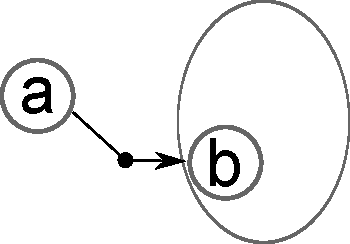
\includegraphics{./fig_exemplo.pdf}
	\end{center}
	\legend{Fonte: \citeonline[p.~12]{meregali}}
\end{figure}

\section{Descrição das Tabelas}
Veja exemplo de formatação da \autoref{tab:exemplo} a seguir: a legenda aparece
acima da tabela, à descrição deve ser centralizada, no número de identificação
2.1, o número 2 corresponde ao capítulo onde se localiza a tabela e o número 1
a ordem da tabela dentro do capítulo, seguido de travessão, espaço e título da
mesma, que deve ter a primeira letra em maiúsculo e o restante em minúsculo.

Observe que as laterais das tabelas são abertas. Isso torna a imagem mais limpa
e clara. As tabelas do texto não devem exceder a margem.

Em relação à referência da tabela, esta deve se localizar na parte inferior da
tabela, precedida da palavra fonte e seguida por dois pontos. Na sequência,
coloca-se o(s) nome(s) da(s) autoria(s) da tabela, seguida do ano e respectiva
página entre parênteses. Exemplo da \autoref{tab:exemplo}:

\begin{table}[htb]
	\centering
		\caption{Exemplo de apresentação de uma tabela no texto}
		\label{tab:exemplo}
		\begin{tabularx}{12cm}{>{\centering}X>{\centering}X X<{\centering}}
		\toprule
			\emph{Manga} & \emph{Abacaxi} & \emph{Morango} \\ \midrule
			12           & 100.000,00     & 10.000,00      \\
			12           & 10.000,00      & 100.000,00     \\ \bottomrule
		\end{tabularx}
		\legend{Fonte: \citeonline[p.~12]{meregali}}
\end{table}

%%%%%%%%%%%%%%%%%%%%%%%%%%%%%%%%%%%%%%%%%%%%%%%%%%%%%%%%%%%%%%

\chapter{Citações}
Há duas formas de se fazer uma citação: a \textbf{citação indireta} ou
\textbf{livre} (também chamada de paráfrase) e a \textbf{citação direta} ou
\textbf{textual}. Pode haver, ainda, a \textbf{citação de citação}. Todas as
citações devem trazer a identificação de sua autoria.

\section{Citação Indireta} A citação indireta ou livre (paráfrase) é aquela
citação na qual se expressa o pensamento de outra pessoa com nossas próprias
palavras. Após fazer a citação, deve-se indicar o nome do autor em letras
minúsculas se estiver no corpo do texto, e com letras maiúsculas se estiver
dentro dos parênteses, juntamente com o ano da publicação da obra em que se
encontra a ideia referida. Não são indicadas páginas já que a ideia pode estar
resumida de uma obra inteira, de um capítulo, de diversas partes ou de um
conjunto delas. Desta forma (com o nome no corpo do texto):

%%% OBS: os framed fazem parte do exemplo, e não devem aparecer no documento final
\begin{framed}
    Depois de analisar a situação, \citeonline{novoa1993} chegou a
    afirmar que o brasileiro ainda não está capacitado para escolher sua
    governante por causa de sua precária vocação política e da absoluta falta
    de escolaridade, já que o homem do povo, o zé-povinho, geralmente não sabe
    sequer em quem votou nas últimas eleições, não sabe sequer quem são seus
    governantes, não saber sequer quem determina seu próprio meio de
    sobreviver.
\end{framed}

Ou, então, com o nome nos parênteses:

\begin{framed}
    Depois de analisar a situação, chegou-se a afirmar que o brasileiro ainda
    não está capacitado para escolher sua governante por causa de sua precária
    vocação política e da absoluta falta de escolaridade, já que o homem do
    povo, o zé-povinho, geralmente não sabe sequer em quem votou nas últimas
    eleições, não sabe sequer quem são seus governantes, não saber sequer quem
    determina seu próprio meio de sobreviver \cite{novoa1993}.
\end{framed}

No caso de o autor possuir outras obras, elas serão diferenciadas pela data da
publicação.  Havendo mais de uma obra no mesmo ano, acrescentamos uma letra
após a data:

\begin{framed}
    No caso do teatro ou do cinema quem melhor se definiu foi
    \citeonline{antunes1997a} quando declarou que aqueles espaços haviam sido
    todos tomados pela geração de 40. Por outro lado, ele próprio se
    contradisse mais tarde (\citeyear{antunes1997b}).
\end{framed}

\section{Citação Direta}
São chamadas de citações diretas ou textuais aquelas em que se transcrevem
exatamente as palavras do autor citado. As citações diretas ou textuais podem
ser breves ou longas. São consideradas breves aquelas cuja extensão não
ultrapassa três linhas. Essas citações devem integrar o texto e devem vir entre
aspas. O tamanho da fonte da citação breve permanece o mesmo do corpo do texto.

\begin{framed}
    Vimos que, para nosso esclarecimento, precisamos seguir os preceitos
    encontrados, já que Guimarães estabelece: ``A valorização da palavra pela
    palavra encarna o objetivo precípuo do texto literário''
    (\citeyear{guim1985}, p.~32) e, se isso não ficar bem esclarecido, nosso
    trabalho será seriamente prejudicado.
\end{framed}

Ou assim:

\begin{framed}
    Vimos que, para nosso esclarecimento, precisamos seguir os preceitos
    encontrados, já que ficou estabelecido que ``A valorização da palavra pela
    palavra encarna o objetivo precípuo do texto literário''
    \cite[p.~32]{guim1985} e, se isso não ficar bem esclarecido, nosso trabalho
    será seriamente prejudicado.
\end{framed}

As citações com mais de três linhas são chamadas de longas e devem receber um
destaque especial com recuo de 4 cm da margem esquerda. Elas não deverão ter
aspas e o tamanho da fonte deve ser menor que o do texto (tamanho 10). A
distância entre as linhas do corpo da citação deve ser de um espaço simples.
Entre o texto da citação e o restante do trabalho, devem-se deixar dois espaços
1,5 cm antes e depois. Exemplo:

\begin{quote}
    Os pronomes O, A, OS e AS passam a serem pronomes demonstrativos sempre que
    numa frase puderem ser substituídos, sem alterar a estrutura dessa frase
    com toda certeza para facilitar a escrita na língua vernácula do próprio
    autor que pensou no seu público de origem. \cite[p.~19]{simoes}
\end{quote}

Havendo supressão de trechos no texto citado, faz-se a indicação com
reticências entre colchetes, denominadas elipses [...]: "Na comunicação diária,
aquela comunicação que utilizamos no dia-a-dia, além da referencialidade da
linguagem [...] há pinceladas de função conativa [...]" \cite[p.~37]{chalhub}.

Em relação à citação de uma citação, é a reprodução de uma informação já citada
por outro autor e, por sua vez, utiliza-se somente na impossibilidade de
consultar o documento original. No texto, deve ser citado o sobrenome do autor
do documento não consultado, seguido da expressão \textbf{apud}, e o nome do
autor do documento consultado. Em nota de rodapé devem ser mencionados os dados
do documento original. Na lista de referências bibliográficas, incluir o
documento efetivamente consultado. Outra opção é incluir as duas referências
dos documentos na lista de referências do trabalho; neste caso, não se inclui
nota de rodapé. A seguir um exemplo com nota de rodapé:


\begin{framed}
	Segundo \apudonline[ p.~5]{franco}{furtado}, texto texto texto texto texto
\end{framed}

ou

\begin{framed}
	texto texto texto texto texto \apud[ p.~5]{franco}{furtado}
\end{framed}



%%%%%%%%%%%%%%%%%%%%%%%%%%%%%%%%%%%%%%%%%%%%%%%%%%%%%%%%%%%%%%
\chapter{Conclusão}

Apresentar conclusão do trabalho xxxx xxxxxx xxxx xxxxx xxxxxxxx xxxxxxx xxxx
xxx xxx xxxxx xxxxxxx xxxx xxxx xxxx xxxxx xxx xxxx xxxxx xxx xx
xxx xxxxxxxx xxxxxxx xxxxx xxxx xxx xxxx xxxx
xxxxxxxx xxxxxxxxxxx xxxxx xxx xxxxxx xxxxx xxxxxxxx xxxx
xxxxxxxxxxxxx xxxx xxxxxxxxxx xxxxxx xxxxxxx xxxxxxxxx xxxx xxx
xxxxx xxxxxxxxxxx xxxxxxxx xxxxx xxxxx xxxxxxx xxxxxxx xxxxx
xxxxxxxxxxxx xxxxxxxxx xxxxxxxx xxxxx xxxxxx xxxxxx xxxxxxxxxxxx

% estes comandos (nocite) servem apenas para que as
% referências abaixo sejam incluídas na bibliografia.

\nocite{goncalves}
\nocite{lisboa}
\nocite{high}
\nocite{krieger}
\nocite{goncalves2}
\nocite{pedrosa}

%%%

\bibliographystyle{abntex2-alf}
\bibliography{bibliografia_exemplo.bib,bibliografia.bib}

\appendix

\chapter*{Descrição do Apêndice}

Destina-se à inclusão de informações complementares ao trabalho, mas que não são essenciais à sua compreensão. Os apêndices devem apresentar material desenvolvido pelo \textbf{próprio autor}, formatado de acordo com a norma NBR 14724. No caso de haver apenas um apêndice, utiliza-se a palavra apêndice no singular.

\annex

\chapter{Descrição do Anexo}

Os anexos destinam-se à inclusão de material como cópias de artigos, manuais, etc., que não necessariamente precisam estar em conformidade com o modelo, e que não foram desenvolvidos pelo autor do trabalho. Nos anexos os números não precisam ser indicados, a não ser na página inicial de cada um. 

\chapter{Exemplo de Anexo}

xxxxxxx xxxx xxxxxxxxxx xxxxxxx xxxx xxxxxxxxxxxxx x xxxxxxx xxxxxxx x xxxxxxx xxxxx xxxxxxxxxxxxxxx xxxxx xxxxxxxx xxxxxxxx xxxxxxxxxxx x xxxx xxxxxx xxxxxxx xxxx xxxxxxxxxxxxxxxxxx xxxxxxx xxxxxxx xxxxxx x xxxxxxxxxxxxxxxxxx xxxxx xxxxxxx xxxxxxxxx xxxxxxxxx xxxxxx xxxxxx xxxxxx xxxxxx xxxxxxxx xxxxxxx xxxx xxxx.


% Os apêndices são um TODO. Parece que há algum problema com eles, inicialmente.
\end{document}
